\documentclass{standalone}
\usepackage{tikz}
\usetikzlibrary{patterns, positioning}


\begin{document}
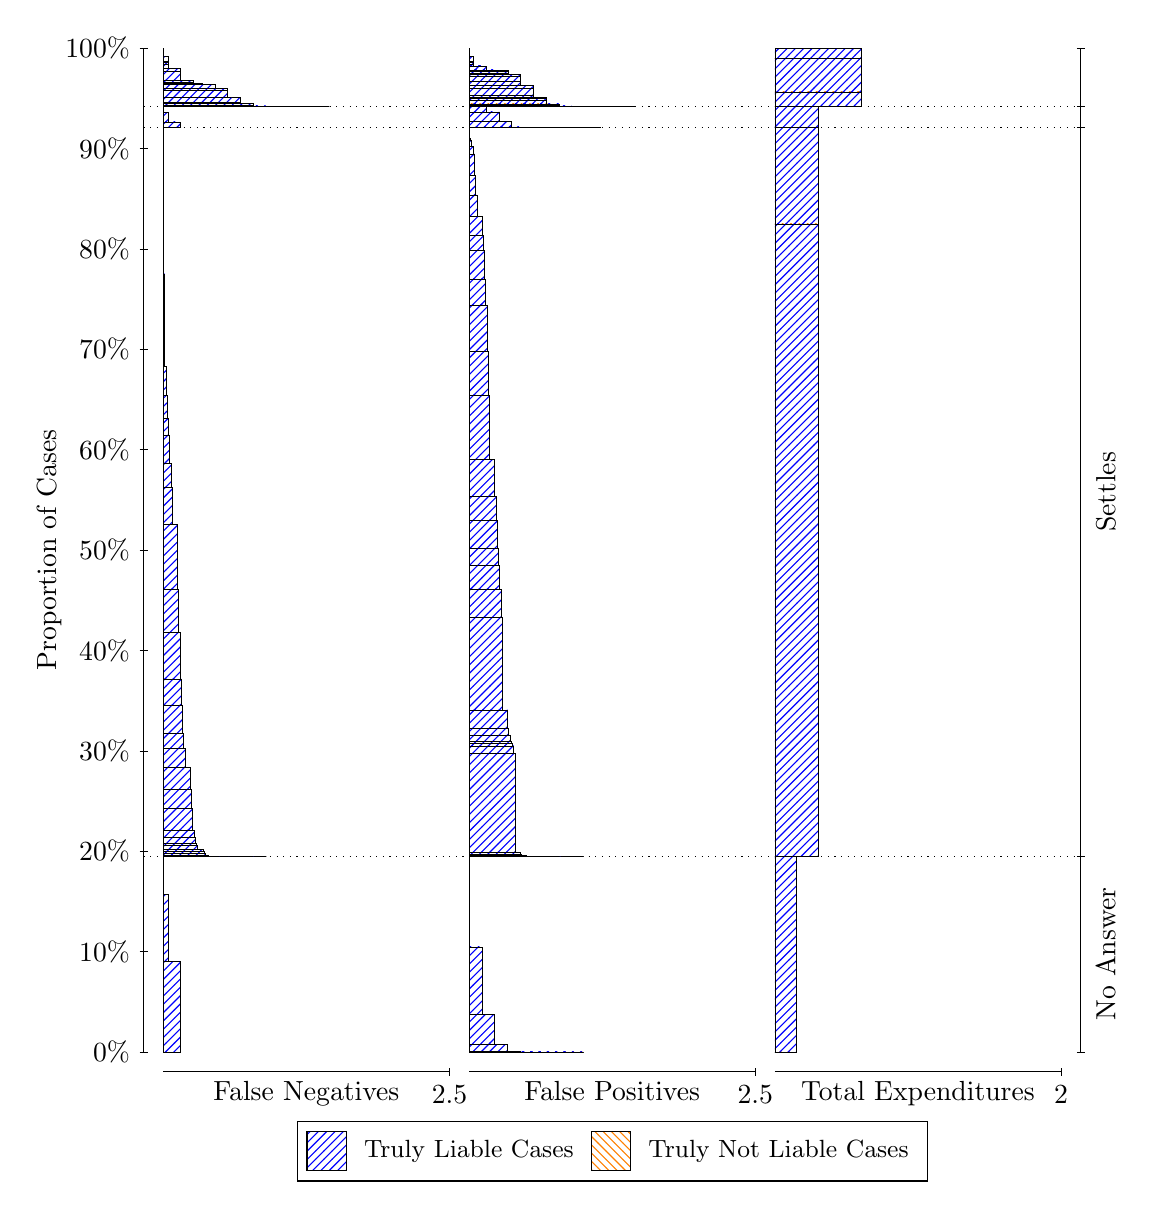
\begin{tikzpicture}
\draw[black, very thin] (1.5,1.75) -- (1.5,14.5);
\node[rotate=90, text=black, anchor=center] at (0.3, 8.125) {Proportion of Cases};
\draw[black, very thin] (1.45,1.75) -- (1.55,1.75);
\node[text=black, anchor=east] at (1.45, 1.75) {0\%};
\draw[black, very thin] (1.45,3.025) -- (1.55,3.025);
\node[text=black, anchor=east] at (1.45, 3.025) {10\%};
\draw[black, very thin] (1.45,4.3) -- (1.55,4.3);
\node[text=black, anchor=east] at (1.45, 4.3) {20\%};
\draw[black, very thin] (1.45,5.575) -- (1.55,5.575);
\node[text=black, anchor=east] at (1.45, 5.575) {30\%};
\draw[black, very thin] (1.45,6.85) -- (1.55,6.85);
\node[text=black, anchor=east] at (1.45, 6.85) {40\%};
\draw[black, very thin] (1.45,8.125) -- (1.55,8.125);
\node[text=black, anchor=east] at (1.45, 8.125) {50\%};
\draw[black, very thin] (1.45,9.4) -- (1.55,9.4);
\node[text=black, anchor=east] at (1.45, 9.4) {60\%};
\draw[black, very thin] (1.45,10.675) -- (1.55,10.675);
\node[text=black, anchor=east] at (1.45, 10.675) {70\%};
\draw[black, very thin] (1.45,11.95) -- (1.55,11.95);
\node[text=black, anchor=east] at (1.45, 11.95) {80\%};
\draw[black, very thin] (1.45,13.225) -- (1.55,13.225);
\node[text=black, anchor=east] at (1.45, 13.225) {90\%};
\draw[black, very thin] (1.45,14.5) -- (1.55,14.5);
\node[text=black, anchor=east] at (1.45, 14.5) {100\%};

\draw[black, very thin] (13.4,1.75) -- (13.4,14.5);
\draw[black, very thin] (13.35,1.75) -- (13.45,1.75);
\node[anchor=west] at (13.35, 1.75) {};
\draw[black, very thin] (13.35,4.2363) -- (13.45,4.2363);
\node[anchor=west] at (13.35, 4.2363) {};
\draw[black, very thin] (13.35,13.489) -- (13.45,13.489);
\node[anchor=west] at (13.35, 13.489) {};
\draw[black, very thin] (13.35,13.761) -- (13.45,13.761);
\node[anchor=west] at (13.35, 13.761) {};
\draw[black, very thin] (13.35,14.5) -- (13.45,14.5);
\node[anchor=west] at (13.35, 14.5) {};

\draw[black, very thin, pattern color=blue, pattern=north east lines] (1.75,1.75) rectangle (1.968,2.9018);
\draw[black, very thin, pattern color=blue, pattern=north east lines] (1.75,2.9018) rectangle (1.8065,3.7553);
\draw[black, very thin, pattern color=orange, pattern=north west lines] (1.75,3.7553) rectangle (1.75,3.7553);
\draw[black, very thin, pattern color=blue, pattern=north east lines] (1.75,3.7553) rectangle (1.75,4.2363);
\draw[black, very thin, pattern color=blue, pattern=north east lines] (1.75,4.2363) rectangle (3.058,4.2363);
\draw[black, very thin, pattern color=blue, pattern=north east lines] (1.75,4.2363) rectangle (2.9127,4.2363);
\draw[black, very thin, pattern color=blue, pattern=north east lines] (1.75,4.2363) rectangle (2.8965,4.2363);
\draw[black, very thin, pattern color=blue, pattern=north east lines] (1.75,4.2363) rectangle (2.7673,4.2363);
\draw[black, very thin, pattern color=blue, pattern=north east lines] (1.75,4.2363) rectangle (2.7512,4.2363);
\draw[black, very thin, pattern color=blue, pattern=north east lines] (1.75,4.2363) rectangle (2.735,4.2363);
\draw[black, very thin, pattern color=blue, pattern=north east lines] (1.75,4.2363) rectangle (2.622,4.2363);
\draw[black, very thin, pattern color=blue, pattern=north east lines] (1.75,4.2363) rectangle (2.6059,4.2363);
\draw[black, very thin, pattern color=blue, pattern=north east lines] (1.75,4.2363) rectangle (2.5897,4.2363);
\draw[black, very thin, pattern color=blue, pattern=north east lines] (1.75,4.2363) rectangle (2.5736,4.2363);
\draw[black, very thin, pattern color=blue, pattern=north east lines] (1.75,4.2363) rectangle (2.4767,4.2364);
\draw[black, very thin, pattern color=blue, pattern=north east lines] (1.75,4.2364) rectangle (2.4605,4.2364);
\draw[black, very thin, pattern color=blue, pattern=north east lines] (1.75,4.2364) rectangle (2.4444,4.237);
\draw[black, very thin, pattern color=blue, pattern=north east lines] (1.75,4.237) rectangle (2.4282,4.2375);
\draw[black, very thin, pattern color=blue, pattern=north east lines] (1.75,4.2375) rectangle (2.4121,4.238);
\draw[black, very thin, pattern color=blue, pattern=north east lines] (1.75,4.238) rectangle (2.3313,4.2391);
\draw[black, very thin, pattern color=blue, pattern=north east lines] (1.75,4.2391) rectangle (2.3152,4.2424);
\draw[black, very thin, pattern color=blue, pattern=north east lines] (1.75,4.2424) rectangle (2.299,4.2478);
\draw[black, very thin, pattern color=blue, pattern=north east lines] (1.75,4.2478) rectangle (2.2829,4.2753);
\draw[black, very thin, pattern color=blue, pattern=north east lines] (1.75,4.2753) rectangle (2.2667,4.3011);
\draw[black, very thin, pattern color=blue, pattern=north east lines] (1.75,4.3011) rectangle (2.2506,4.3274);
\draw[black, very thin, pattern color=blue, pattern=north east lines] (1.75,4.3274) rectangle (2.186,4.3725);
\draw[black, very thin, pattern color=blue, pattern=north east lines] (1.75,4.3725) rectangle (2.1699,4.3993);
\draw[black, very thin, pattern color=blue, pattern=north east lines] (1.75,4.3993) rectangle (2.1537,4.4719);
\draw[black, very thin, pattern color=blue, pattern=north east lines] (1.75,4.4719) rectangle (2.1376,4.57);
\draw[black, very thin, pattern color=blue, pattern=north east lines] (1.75,4.57) rectangle (2.1214,4.8434);
\draw[black, very thin, pattern color=blue, pattern=north east lines] (1.75,4.8434) rectangle (2.1053,5.0892);
\draw[black, very thin, pattern color=blue, pattern=north east lines] (1.75,5.0892) rectangle (2.0891,5.361);
\draw[black, very thin, pattern color=blue, pattern=north east lines] (1.75,5.361) rectangle (2.0245,5.6035);
\draw[black, very thin, pattern color=blue, pattern=north east lines] (1.75,5.6035) rectangle (2.0084,5.7985);
\draw[black, very thin, pattern color=blue, pattern=north east lines] (1.75,5.7985) rectangle (1.9922,6.1574);
\draw[black, very thin, pattern color=blue, pattern=north east lines] (1.75,6.1574) rectangle (1.9761,6.4882);
\draw[black, very thin, pattern color=blue, pattern=north east lines] (1.75,6.4882) rectangle (1.9599,7.0807);
\draw[black, very thin, pattern color=blue, pattern=north east lines] (1.75,7.0807) rectangle (1.9438,7.6315);
\draw[black, very thin, pattern color=blue, pattern=north east lines] (1.75,7.6315) rectangle (1.9276,8.4516);
\draw[black, very thin, pattern color=blue, pattern=north east lines] (1.75,8.4516) rectangle (1.863,8.9162);
\draw[black, very thin, pattern color=blue, pattern=north east lines] (1.75,8.9162) rectangle (1.8469,9.2214);
\draw[black, very thin, pattern color=blue, pattern=north east lines] (1.75,9.2214) rectangle (1.8307,9.5802);
\draw[black, very thin, pattern color=blue, pattern=north east lines] (1.75,9.5802) rectangle (1.8146,9.7989);
\draw[black, very thin, pattern color=blue, pattern=north east lines] (1.75,9.7989) rectangle (1.7984,10.093);
\draw[black, very thin, pattern color=blue, pattern=north east lines] (1.75,10.093) rectangle (1.7823,10.455);
\draw[black, very thin, pattern color=blue, pattern=north east lines] (1.75,10.455) rectangle (1.7661,11.631);
\draw[black, very thin, pattern color=orange, pattern=north west lines] (1.75,11.631) rectangle (1.75,11.631);
\draw[black, very thin, pattern color=blue, pattern=north east lines] (1.75,11.631) rectangle (1.75,13.489);
\draw[black, very thin, pattern color=blue, pattern=north east lines] (1.75,13.489) rectangle (1.968,13.562);
\draw[black, very thin, pattern color=blue, pattern=north east lines] (1.75,13.562) rectangle (1.8065,13.685);
\draw[black, very thin, pattern color=orange, pattern=north west lines] (1.75,13.685) rectangle (1.75,13.685);
\draw[black, very thin, pattern color=blue, pattern=north east lines] (1.75,13.685) rectangle (1.75,13.761);
\draw[black, very thin, pattern color=blue, pattern=north east lines] (1.75,13.761) rectangle (3.8573,13.761);
\draw[black, very thin, pattern color=blue, pattern=north east lines] (1.75,13.761) rectangle (3.6959,13.761);
\draw[black, very thin, pattern color=blue, pattern=north east lines] (1.75,13.761) rectangle (3.5344,13.761);
\draw[black, very thin, pattern color=blue, pattern=north east lines] (1.75,13.761) rectangle (3.5344,13.761);
\draw[black, very thin, pattern color=blue, pattern=north east lines] (1.75,13.761) rectangle (3.3729,13.761);
\draw[black, very thin, pattern color=blue, pattern=north east lines] (1.75,13.761) rectangle (3.2114,13.762);
\draw[black, very thin, pattern color=blue, pattern=north east lines] (1.75,13.762) rectangle (3.0499,13.766);
\draw[black, very thin, pattern color=blue, pattern=north east lines] (1.75,13.766) rectangle (2.9369,13.766);
\draw[black, very thin, pattern color=blue, pattern=north east lines] (1.75,13.766) rectangle (2.8884,13.776);
\draw[black, very thin, pattern color=blue, pattern=north east lines] (1.75,13.776) rectangle (2.8884,13.792);
\draw[black, very thin, pattern color=blue, pattern=north east lines] (1.75,13.792) rectangle (2.7754,13.792);
\draw[black, very thin, pattern color=blue, pattern=north east lines] (1.75,13.792) rectangle (2.7754,13.792);
\draw[black, very thin, pattern color=blue, pattern=north east lines] (1.75,13.792) rectangle (2.727,13.809);
\draw[black, very thin, pattern color=blue, pattern=north east lines] (1.75,13.809) rectangle (2.727,13.873);
\draw[black, very thin, pattern color=blue, pattern=north east lines] (1.75,13.873) rectangle (2.6139,13.873);
\draw[black, very thin, pattern color=blue, pattern=north east lines] (1.75,13.873) rectangle (2.5655,13.963);
\draw[black, very thin, pattern color=blue, pattern=north east lines] (1.75,13.963) rectangle (2.5655,13.989);
\draw[black, very thin, pattern color=blue, pattern=north east lines] (1.75,13.989) rectangle (2.4524,13.989);
\draw[black, very thin, pattern color=blue, pattern=north east lines] (1.75,13.989) rectangle (2.4524,13.989);
\draw[black, very thin, pattern color=blue, pattern=north east lines] (1.75,13.989) rectangle (2.404,14.039);
\draw[black, very thin, pattern color=blue, pattern=north east lines] (1.75,14.039) rectangle (2.291,14.042);
\draw[black, very thin, pattern color=blue, pattern=north east lines] (1.75,14.042) rectangle (2.2425,14.042);
\draw[black, very thin, pattern color=blue, pattern=north east lines] (1.75,14.042) rectangle (2.2425,14.045);
\draw[black, very thin, pattern color=blue, pattern=north east lines] (1.75,14.045) rectangle (2.2425,14.047);
\draw[black, very thin, pattern color=blue, pattern=north east lines] (1.75,14.047) rectangle (2.1295,14.063);
\draw[black, very thin, pattern color=blue, pattern=north east lines] (1.75,14.063) rectangle (2.1295,14.09);
\draw[black, very thin, pattern color=blue, pattern=north east lines] (1.75,14.09) rectangle (2.081,14.091);
\draw[black, very thin, pattern color=blue, pattern=north east lines] (1.75,14.091) rectangle (2.081,14.091);
\draw[black, very thin, pattern color=blue, pattern=north east lines] (1.75,14.091) rectangle (1.968,14.206);
\draw[black, very thin, pattern color=blue, pattern=north east lines] (1.75,14.206) rectangle (1.968,14.238);
\draw[black, very thin, pattern color=blue, pattern=north east lines] (1.75,14.238) rectangle (1.9196,14.238);
\draw[black, very thin, pattern color=blue, pattern=north east lines] (1.75,14.238) rectangle (1.9196,14.238);
\draw[black, very thin, pattern color=blue, pattern=north east lines] (1.75,14.238) rectangle (1.8065,14.29);
\draw[black, very thin, pattern color=blue, pattern=north east lines] (1.75,14.29) rectangle (1.8065,14.316);
\draw[black, very thin, pattern color=blue, pattern=north east lines] (1.75,14.316) rectangle (1.8065,14.329);
\draw[black, very thin, pattern color=blue, pattern=north east lines] (1.75,14.329) rectangle (1.8065,14.392);
\draw[black, very thin, pattern color=blue, pattern=north east lines] (1.75,14.392) rectangle (1.7581,14.392);
\draw[black, very thin, pattern color=blue, pattern=north east lines] (1.75,14.392) rectangle (1.7581,14.392);
\draw[black, very thin, pattern color=orange, pattern=north west lines] (1.75,14.392) rectangle (1.75,14.392);
\draw[black, very thin, pattern color=blue, pattern=north east lines] (1.75,14.392) rectangle (1.75,14.5);
\draw[black, very thin, pattern color=orange, pattern=north west lines] (5.6333,1.75) rectangle (7.0867,1.75);
\draw[black, very thin, pattern color=blue, pattern=north east lines] (5.6333,1.75) rectangle (7.0867,1.75);
\draw[black, very thin, pattern color=blue, pattern=north east lines] (5.6333,1.75) rectangle (6.9252,1.75);
\draw[black, very thin, pattern color=blue, pattern=north east lines] (5.6333,1.75) rectangle (6.7637,1.75);
\draw[black, very thin, pattern color=blue, pattern=north east lines] (5.6333,1.75) rectangle (6.6022,1.75);
\draw[black, very thin, pattern color=blue, pattern=north east lines] (5.6333,1.75) rectangle (6.4407,1.7503);
\draw[black, very thin, pattern color=blue, pattern=north east lines] (5.6333,1.7503) rectangle (6.2793,1.7582);
\draw[black, very thin, pattern color=blue, pattern=north east lines] (5.6333,1.7582) rectangle (6.1178,1.8431);
\draw[black, very thin, pattern color=blue, pattern=north east lines] (5.6333,1.8431) rectangle (5.9563,2.231);
\draw[black, very thin, pattern color=blue, pattern=north east lines] (5.6333,2.231) rectangle (5.7948,3.0845);
\draw[black, very thin, pattern color=blue, pattern=north east lines] (5.6333,3.0845) rectangle (5.6333,4.2363);
\draw[black, very thin, pattern color=orange, pattern=north west lines] (5.6333,4.2363) rectangle (7.0867,4.2363);
\draw[black, very thin, pattern color=blue, pattern=north east lines] (5.6333,4.2363) rectangle (7.0867,4.2363);
\draw[black, very thin, pattern color=orange, pattern=north west lines] (5.6333,4.2363) rectangle (6.9413,4.2363);
\draw[black, very thin, pattern color=blue, pattern=north east lines] (5.6333,4.2363) rectangle (6.9413,4.2363);
\draw[black, very thin, pattern color=blue, pattern=north east lines] (5.6333,4.2363) rectangle (6.9252,4.2363);
\draw[black, very thin, pattern color=orange, pattern=north west lines] (5.6333,4.2363) rectangle (6.796,4.2363);
\draw[black, very thin, pattern color=blue, pattern=north east lines] (5.6333,4.2363) rectangle (6.796,4.2363);
\draw[black, very thin, pattern color=blue, pattern=north east lines] (5.6333,4.2363) rectangle (6.7799,4.2363);
\draw[black, very thin, pattern color=blue, pattern=north east lines] (5.6333,4.2363) rectangle (6.7637,4.2363);
\draw[black, very thin, pattern color=orange, pattern=north west lines] (5.6333,4.2363) rectangle (6.6507,4.2363);
\draw[black, very thin, pattern color=blue, pattern=north east lines] (5.6333,4.2363) rectangle (6.6507,4.2363);
\draw[black, very thin, pattern color=blue, pattern=north east lines] (5.6333,4.2363) rectangle (6.6345,4.2363);
\draw[black, very thin, pattern color=blue, pattern=north east lines] (5.6333,4.2363) rectangle (6.6184,4.2363);
\draw[black, very thin, pattern color=blue, pattern=north east lines] (5.6333,4.2363) rectangle (6.6022,4.2363);
\draw[black, very thin, pattern color=orange, pattern=north west lines] (5.6333,4.2363) rectangle (6.5053,4.2363);
\draw[black, very thin, pattern color=blue, pattern=north east lines] (5.6333,4.2363) rectangle (6.5053,4.2363);
\draw[black, very thin, pattern color=blue, pattern=north east lines] (5.6333,4.2363) rectangle (6.4892,4.2363);
\draw[black, very thin, pattern color=blue, pattern=north east lines] (5.6333,4.2363) rectangle (6.473,4.2364);
\draw[black, very thin, pattern color=blue, pattern=north east lines] (5.6333,4.2364) rectangle (6.4569,4.2364);
\draw[black, very thin, pattern color=blue, pattern=north east lines] (5.6333,4.2364) rectangle (6.4407,4.2369);
\draw[black, very thin, pattern color=orange, pattern=north west lines] (5.6333,4.2369) rectangle (6.36,4.2369);
\draw[black, very thin, pattern color=blue, pattern=north east lines] (5.6333,4.2369) rectangle (6.36,4.2484);
\draw[black, very thin, pattern color=blue, pattern=north east lines] (5.6333,4.2484) rectangle (6.3439,4.2493);
\draw[black, very thin, pattern color=blue, pattern=north east lines] (5.6333,4.2493) rectangle (6.3277,4.2501);
\draw[black, very thin, pattern color=blue, pattern=north east lines] (5.6333,4.2501) rectangle (6.3116,4.2529);
\draw[black, very thin, pattern color=blue, pattern=north east lines] (5.6333,4.2529) rectangle (6.2954,4.2581);
\draw[black, very thin, pattern color=blue, pattern=north east lines] (5.6333,4.2581) rectangle (6.2793,4.2833);
\draw[black, very thin, pattern color=orange, pattern=north west lines] (5.6333,4.2833) rectangle (6.2147,4.2833);
\draw[black, very thin, pattern color=blue, pattern=north east lines] (5.6333,4.2833) rectangle (6.2147,5.5464);
\draw[black, very thin, pattern color=blue, pattern=north east lines] (5.6333,5.5464) rectangle (6.1985,5.6367);
\draw[black, very thin, pattern color=blue, pattern=north east lines] (5.6333,5.6367) rectangle (6.1824,5.6699);
\draw[black, very thin, pattern color=blue, pattern=north east lines] (5.6333,5.6699) rectangle (6.1662,5.6987);
\draw[black, very thin, pattern color=blue, pattern=north east lines] (5.6333,5.6987) rectangle (6.1501,5.7704);
\draw[black, very thin, pattern color=blue, pattern=north east lines] (5.6333,5.7704) rectangle (6.1339,5.8636);
\draw[black, very thin, pattern color=blue, pattern=north east lines] (5.6333,5.8636) rectangle (6.1178,6.0948);
\draw[black, very thin, pattern color=blue, pattern=north east lines] (5.6333,6.0948) rectangle (6.0532,7.2707);
\draw[black, very thin, pattern color=blue, pattern=north east lines] (5.6333,7.2707) rectangle (6.037,7.6325);
\draw[black, very thin, pattern color=blue, pattern=north east lines] (5.6333,7.6325) rectangle (6.0209,7.9268);
\draw[black, very thin, pattern color=blue, pattern=north east lines] (5.6333,7.9268) rectangle (6.0047,8.1455);
\draw[black, very thin, pattern color=blue, pattern=north east lines] (5.6333,8.1455) rectangle (5.9886,8.5043);
\draw[black, very thin, pattern color=blue, pattern=north east lines] (5.6333,8.5043) rectangle (5.9724,8.8094);
\draw[black, very thin, pattern color=blue, pattern=north east lines] (5.6333,8.8094) rectangle (5.9563,9.2741);
\draw[black, very thin, pattern color=blue, pattern=north east lines] (5.6333,9.2741) rectangle (5.8917,10.094);
\draw[black, very thin, pattern color=blue, pattern=north east lines] (5.6333,10.094) rectangle (5.8756,10.645);
\draw[black, very thin, pattern color=blue, pattern=north east lines] (5.6333,10.645) rectangle (5.8594,11.237);
\draw[black, very thin, pattern color=blue, pattern=north east lines] (5.6333,11.237) rectangle (5.8433,11.568);
\draw[black, very thin, pattern color=blue, pattern=north east lines] (5.6333,11.568) rectangle (5.8271,11.927);
\draw[black, very thin, pattern color=blue, pattern=north east lines] (5.6333,11.927) rectangle (5.811,12.122);
\draw[black, very thin, pattern color=blue, pattern=north east lines] (5.6333,12.122) rectangle (5.7948,12.365);
\draw[black, very thin, pattern color=blue, pattern=north east lines] (5.6333,12.365) rectangle (5.7302,12.636);
\draw[black, very thin, pattern color=blue, pattern=north east lines] (5.6333,12.636) rectangle (5.7141,12.882);
\draw[black, very thin, pattern color=blue, pattern=north east lines] (5.6333,12.882) rectangle (5.6979,13.156);
\draw[black, very thin, pattern color=blue, pattern=north east lines] (5.6333,13.156) rectangle (5.6818,13.254);
\draw[black, very thin, pattern color=blue, pattern=north east lines] (5.6333,13.254) rectangle (5.6656,13.326);
\draw[black, very thin, pattern color=blue, pattern=north east lines] (5.6333,13.326) rectangle (5.6495,13.353);
\draw[black, very thin, pattern color=blue, pattern=north east lines] (5.6333,13.353) rectangle (5.6333,13.489);
\draw[black, very thin, pattern color=orange, pattern=north west lines] (5.6333,13.489) rectangle (7.3047,13.489);
\draw[black, very thin, pattern color=blue, pattern=north east lines] (5.6333,13.489) rectangle (7.3047,13.489);
\draw[black, very thin, pattern color=blue, pattern=north east lines] (5.6333,13.489) rectangle (7.1432,13.489);
\draw[black, very thin, pattern color=blue, pattern=north east lines] (5.6333,13.489) rectangle (6.9817,13.489);
\draw[black, very thin, pattern color=blue, pattern=north east lines] (5.6333,13.489) rectangle (6.8202,13.489);
\draw[black, very thin, pattern color=blue, pattern=north east lines] (5.6333,13.489) rectangle (6.6587,13.489);
\draw[black, very thin, pattern color=blue, pattern=north east lines] (5.6333,13.489) rectangle (6.4973,13.49);
\draw[black, very thin, pattern color=blue, pattern=north east lines] (5.6333,13.49) rectangle (6.3358,13.499);
\draw[black, very thin, pattern color=blue, pattern=north east lines] (5.6333,13.499) rectangle (6.1743,13.565);
\draw[black, very thin, pattern color=blue, pattern=north east lines] (5.6333,13.565) rectangle (6.0128,13.689);
\draw[black, very thin, pattern color=blue, pattern=north east lines] (5.6333,13.689) rectangle (5.8513,13.761);
\draw[black, very thin, pattern color=orange, pattern=north west lines] (5.6333,13.761) rectangle (7.7407,13.761);
\draw[black, very thin, pattern color=blue, pattern=north east lines] (5.6333,13.761) rectangle (7.7407,13.761);
\draw[black, very thin, pattern color=orange, pattern=north west lines] (5.6333,13.761) rectangle (7.5792,13.761);
\draw[black, very thin, pattern color=blue, pattern=north east lines] (5.6333,13.761) rectangle (7.5792,13.761);
\draw[black, very thin, pattern color=orange, pattern=north west lines] (5.6333,13.761) rectangle (7.4177,13.761);
\draw[black, very thin, pattern color=blue, pattern=north east lines] (5.6333,13.761) rectangle (7.4177,13.761);
\draw[black, very thin, pattern color=blue, pattern=north east lines] (5.6333,13.761) rectangle (7.4177,13.761);
\draw[black, very thin, pattern color=orange, pattern=north west lines] (5.6333,13.761) rectangle (7.2562,13.761);
\draw[black, very thin, pattern color=blue, pattern=north east lines] (5.6333,13.761) rectangle (7.2562,13.761);
\draw[black, very thin, pattern color=orange, pattern=north west lines] (5.6333,13.761) rectangle (7.0947,13.761);
\draw[black, very thin, pattern color=blue, pattern=north east lines] (5.6333,13.761) rectangle (7.0947,13.761);
\draw[black, very thin, pattern color=orange, pattern=north west lines] (5.6333,13.761) rectangle (6.9817,13.761);
\draw[black, very thin, pattern color=blue, pattern=north east lines] (5.6333,13.761) rectangle (6.9817,13.761);
\draw[black, very thin, pattern color=blue, pattern=north east lines] (5.6333,13.761) rectangle (6.9333,13.763);
\draw[black, very thin, pattern color=blue, pattern=north east lines] (5.6333,13.763) rectangle (6.9333,13.763);
\draw[black, very thin, pattern color=orange, pattern=north west lines] (5.6333,13.763) rectangle (6.9333,13.763);
\draw[black, very thin, pattern color=blue, pattern=north east lines] (5.6333,13.763) rectangle (6.9333,13.765);
\draw[black, very thin, pattern color=orange, pattern=north west lines] (5.6333,13.765) rectangle (6.8202,13.765);
\draw[black, very thin, pattern color=blue, pattern=north east lines] (5.6333,13.765) rectangle (6.8202,13.765);
\draw[black, very thin, pattern color=blue, pattern=north east lines] (5.6333,13.765) rectangle (6.7718,13.775);
\draw[black, very thin, pattern color=blue, pattern=north east lines] (5.6333,13.775) rectangle (6.7718,13.783);
\draw[black, very thin, pattern color=orange, pattern=north west lines] (5.6333,13.783) rectangle (6.7718,13.783);
\draw[black, very thin, pattern color=blue, pattern=north east lines] (5.6333,13.783) rectangle (6.7718,13.79);
\draw[black, very thin, pattern color=orange, pattern=north west lines] (5.6333,13.79) rectangle (6.6587,13.79);
\draw[black, very thin, pattern color=blue, pattern=north east lines] (5.6333,13.79) rectangle (6.6587,13.79);
\draw[black, very thin, pattern color=blue, pattern=north east lines] (5.6333,13.79) rectangle (6.6587,13.79);
\draw[black, very thin, pattern color=blue, pattern=north east lines] (5.6333,13.79) rectangle (6.6103,13.834);
\draw[black, very thin, pattern color=blue, pattern=north east lines] (5.6333,13.834) rectangle (6.6103,13.868);
\draw[black, very thin, pattern color=blue, pattern=north east lines] (5.6333,13.868) rectangle (6.6103,13.869);
\draw[black, very thin, pattern color=blue, pattern=north east lines] (5.6333,13.869) rectangle (6.4973,13.869);
\draw[black, very thin, pattern color=orange, pattern=north west lines] (5.6333,13.869) rectangle (6.4973,13.869);
\draw[black, very thin, pattern color=blue, pattern=north east lines] (5.6333,13.869) rectangle (6.4973,13.869);
\draw[black, very thin, pattern color=blue, pattern=north east lines] (5.6333,13.869) rectangle (6.4488,13.902);
\draw[black, very thin, pattern color=blue, pattern=north east lines] (5.6333,13.902) rectangle (6.4488,13.992);
\draw[black, very thin, pattern color=blue, pattern=north east lines] (5.6333,13.992) rectangle (6.4488,14.023);
\draw[black, very thin, pattern color=blue, pattern=north east lines] (5.6333,14.023) rectangle (6.3358,14.023);
\draw[black, very thin, pattern color=blue, pattern=north east lines] (5.6333,14.023) rectangle (6.3358,14.023);
\draw[black, very thin, pattern color=orange, pattern=north west lines] (5.6333,14.023) rectangle (6.3358,14.023);
\draw[black, very thin, pattern color=blue, pattern=north east lines] (5.6333,14.023) rectangle (6.3358,14.023);
\draw[black, very thin, pattern color=blue, pattern=north east lines] (5.6333,14.023) rectangle (6.2873,14.08);
\draw[black, very thin, pattern color=blue, pattern=north east lines] (5.6333,14.08) rectangle (6.2873,14.138);
\draw[black, very thin, pattern color=blue, pattern=north east lines] (5.6333,14.138) rectangle (6.2873,14.17);
\draw[black, very thin, pattern color=blue, pattern=north east lines] (5.6333,14.17) rectangle (6.1743,14.17);
\draw[black, very thin, pattern color=orange, pattern=north west lines] (5.6333,14.17) rectangle (6.1743,14.17);
\draw[black, very thin, pattern color=blue, pattern=north east lines] (5.6333,14.17) rectangle (6.1743,14.171);
\draw[black, very thin, pattern color=blue, pattern=north east lines] (5.6333,14.171) rectangle (6.1743,14.171);
\draw[black, very thin, pattern color=blue, pattern=north east lines] (5.6333,14.171) rectangle (6.1259,14.173);
\draw[black, very thin, pattern color=blue, pattern=north east lines] (5.6333,14.173) rectangle (6.1259,14.199);
\draw[black, very thin, pattern color=blue, pattern=north east lines] (5.6333,14.199) rectangle (6.1259,14.214);
\draw[black, very thin, pattern color=blue, pattern=north east lines] (5.6333,14.214) rectangle (6.0128,14.216);
\draw[black, very thin, pattern color=blue, pattern=north east lines] (5.6333,14.216) rectangle (6.0128,14.219);
\draw[black, very thin, pattern color=orange, pattern=north west lines] (5.6333,14.219) rectangle (6.0128,14.219);
\draw[black, very thin, pattern color=blue, pattern=north east lines] (5.6333,14.219) rectangle (6.0128,14.219);
\draw[black, very thin, pattern color=blue, pattern=north east lines] (5.6333,14.219) rectangle (5.9644,14.22);
\draw[black, very thin, pattern color=blue, pattern=north east lines] (5.6333,14.22) rectangle (5.9644,14.221);
\draw[black, very thin, pattern color=blue, pattern=north east lines] (5.6333,14.221) rectangle (5.9644,14.222);
\draw[black, very thin, pattern color=blue, pattern=north east lines] (5.6333,14.222) rectangle (5.8513,14.268);
\draw[black, very thin, pattern color=orange, pattern=north west lines] (5.6333,14.268) rectangle (5.8513,14.268);
\draw[black, very thin, pattern color=blue, pattern=north east lines] (5.6333,14.268) rectangle (5.8513,14.269);
\draw[black, very thin, pattern color=blue, pattern=north east lines] (5.6333,14.269) rectangle (5.8513,14.272);
\draw[black, very thin, pattern color=blue, pattern=north east lines] (5.6333,14.272) rectangle (5.8029,14.272);
\draw[black, very thin, pattern color=blue, pattern=north east lines] (5.6333,14.272) rectangle (5.8029,14.272);
\draw[black, very thin, pattern color=blue, pattern=north east lines] (5.6333,14.272) rectangle (5.6899,14.298);
\draw[black, very thin, pattern color=blue, pattern=north east lines] (5.6333,14.298) rectangle (5.6899,14.325);
\draw[black, very thin, pattern color=blue, pattern=north east lines] (5.6333,14.325) rectangle (5.6899,14.327);
\draw[black, very thin, pattern color=blue, pattern=north east lines] (5.6333,14.327) rectangle (5.6899,14.389);
\draw[black, very thin, pattern color=blue, pattern=north east lines] (5.6333,14.389) rectangle (5.6414,14.389);
\draw[black, very thin, pattern color=blue, pattern=north east lines] (5.6333,14.389) rectangle (5.6414,14.389);
\draw[black, very thin, pattern color=blue, pattern=north east lines] (5.6333,14.389) rectangle (5.6333,14.5);
\draw[black, very thin, pattern color=orange, pattern=north west lines] (9.5167,1.75) rectangle (9.7892,1.75);
\draw[black, very thin, pattern color=blue, pattern=north east lines] (9.5167,1.75) rectangle (9.7892,4.2363);
\draw[black, very thin, pattern color=orange, pattern=north west lines] (9.5167,4.2363) rectangle (10.062,4.2363);
\draw[black, very thin, pattern color=blue, pattern=north east lines] (9.5167,4.2363) rectangle (10.062,12.267);
\draw[black, very thin, pattern color=orange, pattern=north west lines] (9.5167,12.267) rectangle (10.062,12.267);
\draw[black, very thin, pattern color=blue, pattern=north east lines] (9.5167,12.267) rectangle (10.062,13.489);
\draw[black, very thin, pattern color=orange, pattern=north west lines] (9.5167,13.489) rectangle (10.062,13.489);
\draw[black, very thin, pattern color=blue, pattern=north east lines] (9.5167,13.489) rectangle (10.062,13.761);
\draw[black, very thin, pattern color=orange, pattern=north west lines] (9.5167,13.761) rectangle (10.607,13.761);
\draw[black, very thin, pattern color=blue, pattern=north east lines] (9.5167,13.761) rectangle (10.607,13.943);
\draw[black, very thin, pattern color=orange, pattern=north west lines] (9.5167,13.943) rectangle (10.607,13.943);
\draw[black, very thin, pattern color=blue, pattern=north east lines] (9.5167,13.943) rectangle (10.607,14.368);
\draw[black, very thin, pattern color=orange, pattern=north west lines] (9.5167,14.368) rectangle (10.607,14.368);
\draw[black, very thin, pattern color=blue, pattern=north east lines] (9.5167,14.368) rectangle (10.607,14.5);
\draw[black, dotted] (1.5,4.2363) -- (13.4,4.2363);
\draw[black, dotted] (1.5,13.489) -- (13.4,13.489);
\draw[black, dotted] (1.5,13.761) -- (13.4,13.761);
\draw[black, very thin] (1.75,1.5) -- (5.3833,1.5);
\node[text=black, anchor=north] at (3.5667, 1.5) {False Negatives};
\draw[black, very thin] (5.3833,1.45) -- (5.3833,1.55);
\node[text=black, anchor=north] at (5.3833, 1.45) {2.5};

\draw[black, very thin] (5.6333,1.5) -- (9.2667,1.5);
\node[text=black, anchor=north] at (7.45, 1.5) {False Positives};
\draw[black, very thin] (9.2667,1.45) -- (9.2667,1.55);
\node[text=black, anchor=north] at (9.2667, 1.45) {2.5};

\draw[black, very thin] (9.5167,1.5) -- (13.15,1.5);
\node[text=black, anchor=north] at (11.333, 1.5) {Total Expenditures};
\draw[black, very thin] (13.15,1.45) -- (13.15,1.55);
\node[text=black, anchor=north] at (13.15, 1.45) {2};

\node[text=black, centered, rotate=90] at (13.72, 2.9932) {No Answer};
\node[text=black, centered, rotate=90] at (13.72, 8.8628) {Settles};



\draw (7.449999999999999,1.5) node[draw=none] (baseCoordinate) {};
\begin{scope}[align=center]
        \matrix[scale=0.5, draw=black, below=0.5cm of baseCoordinate, nodes={draw}, column sep=0.1cm]{
            \node[rectangle, draw, minimum width=0.5cm, minimum height=0.5cm, pattern color=blue, pattern=north east lines] {}; &
            \node[draw=none, font=\small, text=black] (B) {Truly Liable Cases}; &
            \node[rectangle, draw, minimum width=0.5cm, minimum height=0.5cm, pattern color=orange, pattern=north west lines] {}; &
            \node[draw=none, font=\small, text=black] (B) {Truly Not Liable Cases}; \\
            };
\end{scope}

\end{tikzpicture}
\end{document}